\chapter{Time Projection Chamber}
\label{sec:tpc}
	A~\acf{TPC} is a~gaseous detector that uses the drift times of ionization electrons produced by a~charged particle in an (ideally uniform) electric field to reconstruct the particle's 3D~trajectory. The 2D~projection is measured by an amplification stage at the end of the drift volume. When placed inside a~magnetic field (typically parallel to the electric field), the momentum of the incident particle can be inferred from the curvature of its trajectory. Particle identification is also possible using the ionization energy loss inside the \ac{TPC} (see \cref{fig:particleid}). The following text (including \cref{sec:transport,sec:readout}) is based primarily on the reviews by Hilke~\cite{TPCs} and the Particle Data Group~\cite{pdg2024}.
	
	\begin{figure}[H]
		\centering
		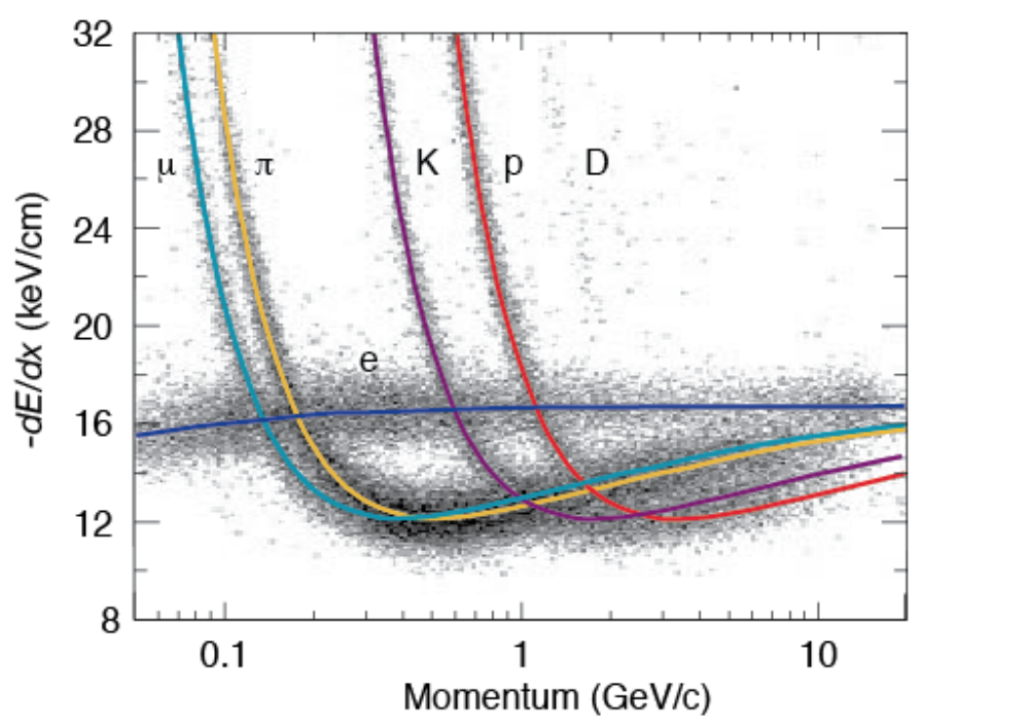
\includegraphics[width=0.6\textwidth]{particle_id.png}
		\caption{Particle identification in the PEP-4 \ac{TPC} at SLAC based on the energy loss per distance $\dv{E}{x}$ in the 80:20 Ar:CH$_4$ filling at \qty{8.5}{atm} pressure~\cite{particleid}.\orange{~The reference doesn't point to the original PEP-4 article because this adapted version of the original picture that they used in the DUNE article looks better.}}
		\label{fig:particleid}
	\end{figure}
	
	Large \acp{TPC} are sensitive to small distortions in the electric field (imperfections in the field cage, accumulation of positive ions in the gas volume) and to $\mathbf{E}\cross\mathbf{B}$ effects on the drift velocity (see \cref{eq:drift} below). Diffusion of the drifting electrons deteriorates the spacial resolution significantly, but it can be reduced up to \textapprox10~times by a~strong $\mathbf{B}\parallel\mathbf{E}$ field (see \cref{eq:difmag}).
	
	In neutrino and other rare-event experiments, large (up to 600 tons) \acp{LArTPC} are used for particle identification and calorimetry. The ionization electrons can be drifted for many meters with a~small diffusion. Scintillation photons are also measured.\red{~Negative ions?}
	
	\section{Charge transport in gases}
	\label{sec:transport}
		When a~charged particle crosses the volume of a~\ac{TPC}, it loses energy by excitation and ionization of the detector gas\red{~(how much -- from dE/dx + density $\rightarrow$ footnote?)}. Most ionizing collision produce a~single ionization electron, sometimes a~few secondary electrons are produced near the collision vertex, creating a~cluster. In rare cases, the ionization electron has energy large enough to create a measurable track, such an electron is called a~$\delta$\nobreakdash-electron\orange{~(terminology, just like bellow -- technically it's a (primary) ionization electron causing other (secondary) ionization)}.
		
		After their release, the ionization electrons are separated from positive ions by the electric field and they both drift and diffuse in opposite directions towards the electrodes. The charges are accelerated\orange{~(different word?)} by the electric field inside the chamber, and they lose speed by colliding with the gas particles, quickly reaching a~constant (for a~given field $\mathbf{E}, \mathbf{B}$) mean drift velocity. The electrons can be absorbed by electronegative impurities, such as halides, O$_2$, and H$_2$O.
		
		In mixtures with a~noble gas component, if the excitation energy of the noble gas is higher then the ionization potential of an admixture, more free electrons can be produced through collisions of the gas particles (so\nobreakdash-called Penning transfer) and through absorption of emitted photons.
		
		If the electric field is strong enough, the electrons can cause further ionization and excitation of the gas, leading to the development of a~Townsend avalanche\red{~(ref)}.
	
		\subsection{Drift}			
			In many gases (called "hot", e.g., Ar or CH$_4$), the drift velocity is much greater than that of their thermal motion thanks to a~high proportion of elastic collisions. On the other hand, "cold" gases like CO$_2$ have a higher proportion of inelastic collisions (e.g., thanks to the excitation of rotational and vibrational states) and therefore much lower\orange{~(value? magnitude (implied)?)} drift velocity.\red{~Or maybe it is not so simple, because slowing down the electrons inelastically into a certain minimum of elastic scattering cross-section increases drift velocity? In case of Ar+CO$_2$ this is clearly not the case for low electric fields, so maybe irrelevant here (or is the effect opposite for small additions?).}
			
			The ions produced by the ionization lose a significant portion of their energy during each collision since their mass is close to the mass of the gas particles\orange{~(see the source material -- average energy loss during collision $\Delta E = \frac{2m_i M}{(m_i+M)^2}$, this way it's more accurate)}. This, together with their large collision cross section, makes their drift velocity much smaller (about three orders of magnitude) and their energy is close to thermal. Since their momenta are not randomized to such an extent during collisions, their diffusion is smaller\red{~(move this to the diffusion subsection, reformulate)}.
			
			The drift is also influenced by the magnetic field. Langevin derived a~good approximation for the drift velocity vector:
				\begin{equation}
					\label{eq:drift}
					\mathbf{v}_\text{d} = \left(\frac{\mathbf{E}}{\norm{\mathbf{E}}} + \omega\tau\frac{\mathbf{E}\times\mathbf{B}}{\norm{\mathbf{E}}\norm{\mathbf{B}}} + \omega^2\tau^2\frac{\mathbf{E}\cdot\mathbf{B}}{\norm{\mathbf{E}}\norm{\mathbf{B}}}\cdot \frac{\mathbf{B}}{\norm{\mathbf{B}}}\right) \frac{q\tau}{m(1+\omega^2\tau^2)}\norm{\mathbf{E}},
				\end{equation}
			where $q$ is the charge of the particle, $m$ is its mass, $\tau$ is the mean time between collisions and $\omega = \frac{q}{m}\norm{\mathbf{B}}$ is the Larmor frequency. For orthogonal fields $\mathbf{E}\perp\mathbf{B}$, it can be shown that the magnetic field bends the direction of the drift by the so\nobreakdash-called Lorentz angle:
				\begin{equation}
					\label{eq:lorentz}
					\tan\psi = -\omega\tau.
				\end{equation}
			The drift of ions is only negligibly influenced by the magnetic field ($\omega\tau\sim10^{-4}$ is small due to the low drift velocity\orange{~-- better (?) because it takes $\tau$ into account and differs only by E/B ratio (if the magnetic contribution to the magnitude is small)}). In a~standard \ac{TPC}, $\mathbf{E}$ is parallel to $\mathbf{B}$ and the influence of the magnetic field on the drift is minimal. Without magnetic field, we can write
				\begin{equation}
					\mathbf{v}_d = \frac{q\tau}{m} \mathbf{E} = \mu \mathbf{E},
				\end{equation}
			where $\mu$ is called charge mobility.
			
		\subsection{Diffusion}
			\orange{All of the theory is from the same source mentioned at the beginning. None of the simulations explicitly depend on this.}
			Due to collisions, a~cloud of electrons or ions originating from the same point will show a~Gaussian density distribution at time $t$ while drifting in the electric field $\mathbf{E} = (0,0,E_z)$ along the $z$\nobreakdash-coordinate\orange{~(coordinates defined by the electric field)}:
				\begin{equation}
					\rho(x,y,z,t) = (4\pi Dt)^{-\frac{3}{2}} \exp\left(-\frac{x^2+y^2+(z-v_dt)^2}{4Dt}\right),
				\end{equation}
			where the diffusion coefficient $D$ can be expressed as
				\begin{equation}
					D = \frac{\lambda^2}{3\tau} = \frac{\lambda v_\text{d}}{3} = \frac{v_\text{d}^2\tau}{3} = \frac{2\varepsilon\tau}{3m},
				\end{equation}
			where $\lambda$ is the mean free path and $\varepsilon$ the mean kinetic energy. The lateral diffusion width $\sigma_x$ after a drift distance $L$ can be expressed as
				\begin{equation}
					\sigma_x^2 = 2Dt = \frac{4\varepsilon L}{3qE_z}.
				\end{equation}
			The minimal diffusion width is given by the lowest possible energy of the particles $\varepsilon_\text{th} = \frac{3}{2}kT$ (corresponding to thermal motion):
				\begin{equation}
					\sigma_{x, \,\text{min}}^2 = \frac{2kTL}{qE}.
				\end{equation}
			For electrons in "cold gases" (e.g., Ar/CO$_2$ mixture), the diffusion approaches this limit up to a~certain field intensity (\textapprox\qty{100}{\V\per\cm} at 1~atm pressure)\footnote{\red{For us $\sigma_{x, \,\text{min}} = 0.45$~mm, quite close to the actual diffusion 0.5-0.7~mm -- details of the calculation.}}. In reality, the transversal diffusion of electrons can differ significantly from their longitudinal diffusion and simulations are necessary to get a~precise result.
			
			In most \acp{TPC}, the transversal (but not the longitudinal) diffusion is reduced by the magnetic field, since it is parallel to the electric field and curves the diffusing electrons around their mean trajectory:
				\begin{equation}
					\label{eq:difmag}
					\frac{D_\text{T}(B)}{D_\text{T}(0)} = \frac{1}{C+\omega^2\tau_2^2},
				\end{equation}
			where $C$ and $\tau_2$ are parameters dependent on the gas used. At low intensity of the magnetic field, we can use an approximation $C\approx1$ and $\tau_2\approx\tau$.
			
	\section{Examples of TPCs}
		\subsection{The original TPC at PEP-4 at SLAC}
			The original \ac{TPC} used in the PEP-4 experiment at SLAC in the 1980s (\cref{fig:pep4}) was a \qtyproduct[product-units=repeat]{2x2}{\m} hollow cylinder with a~central cathode that produced a~strong electric field \qty{750}{\V\per\cm}, making the ionization electrons drift towards one of the endcaps~\cite{pep4-2}. It was filled with a~80:20 Ar:CH$_4$ mixture at \qty{8.5}{atm} pressure and placed inside a~\qty{0.4}{\tesla} solenoidal magnetic field. The readout consisted of \acp{MWPC}, where electrons are accelerated towards the anode wires fast enough to further ionize the gas and cause an avalanche (details are provided in \cref{sec:MWPC}). The wires had radial spacing \qty{4}{\mm}, fifteen of the sense wires had the cathode segmented into \qtyproduct{7.0x7.5}{\mm} pads \qty{4}{\mm} under them (\cref{fig:pep4} right). When collecting electrons on the anode wire, signal is induced on the nearest \numrange{2}{3} cathode pads.
			
			\begin{figure}
				\centering
				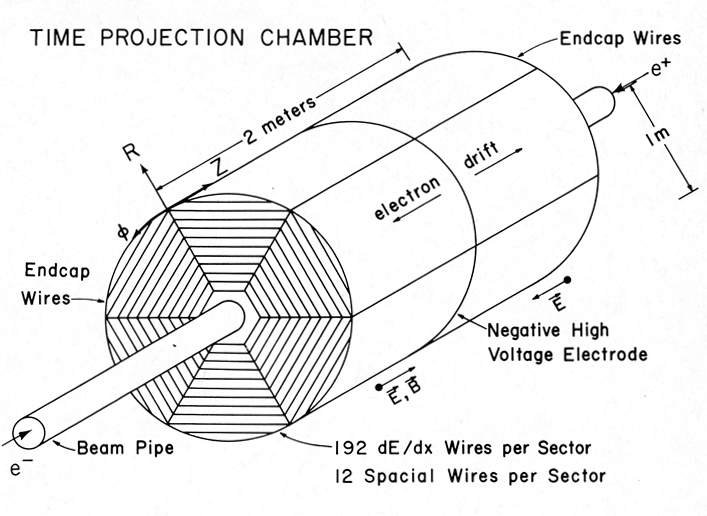
\includegraphics[width=0.6\textwidth]{pep4_tpc.png}
				\hfill
				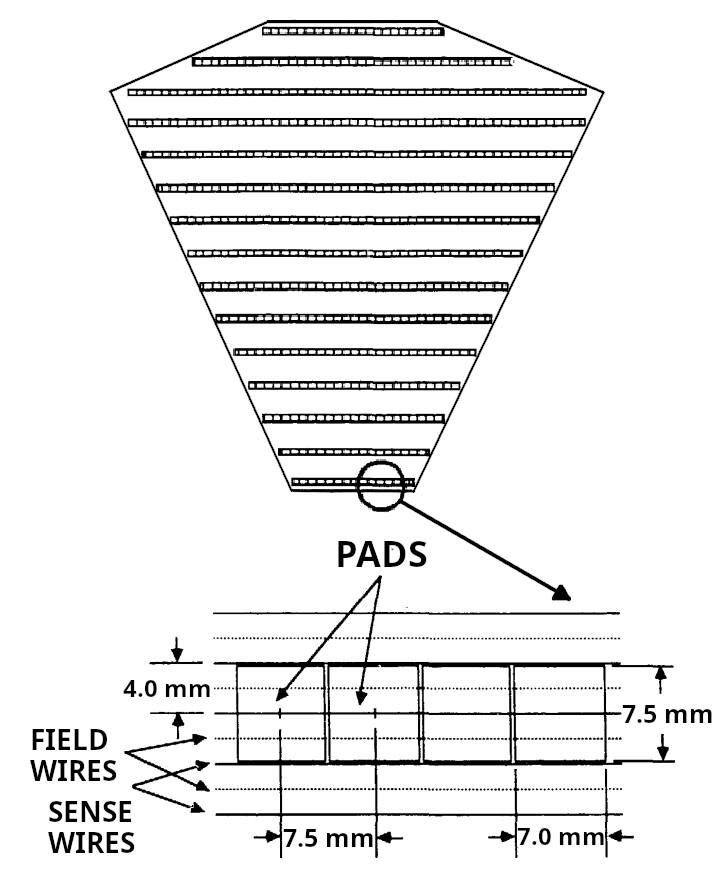
\includegraphics[width=0.38\textwidth]{pep4_readout_edit.png}
				\caption{Schematic view of the PEP-4 \ac{TPC}~\cite{pep4}. A~charged particle produced in a~collision in the beam pipe creates a~spiral ionization track in the magnetic field. The central cathode then accelerates ionization electrons towards the endcap anode wires where they are multiplied and read out. A~\ac{TPC} sector with a~detailed view of one of the pad rows is shown on the right~\cite{pep4_readout}.}
				\label{fig:pep4}
			\end{figure}
		
		\subsection{ALICE TPC}
			The ALICE \ac{TPC} (\cref{fig:alice}) is the main detector used for charged particle tracking and recognition in collisions at the ALICE experiment at the CERN LHC~\cite{ALICE}. Similarly to PEP\nobreakdash-4, it is a hollow cylinder with outer radius \qty{2.5}{\m} and height \qty{5}{\m}. It is placed in a~\qty{0.5}{\tesla} solenoidal magnetic field, and the central cathode generates a~\qty{400}{\V\per\cm} electric field inside the field cage. The gas mixture in the detector is 90:10:5 Ne:CO$_2$:N$_2$, mainly chosen for its higher ion mobility compared to Ar mixtures. In 2020, the readout of the \ac{TPC} was upgraded from \acp{MWPC} to stacks of four \ac{GEM} foils (principle described in \cref{sec:mpgd}). This allows reading events continuously at a~higher rate.
			
			\begin{figure}
				\centering
				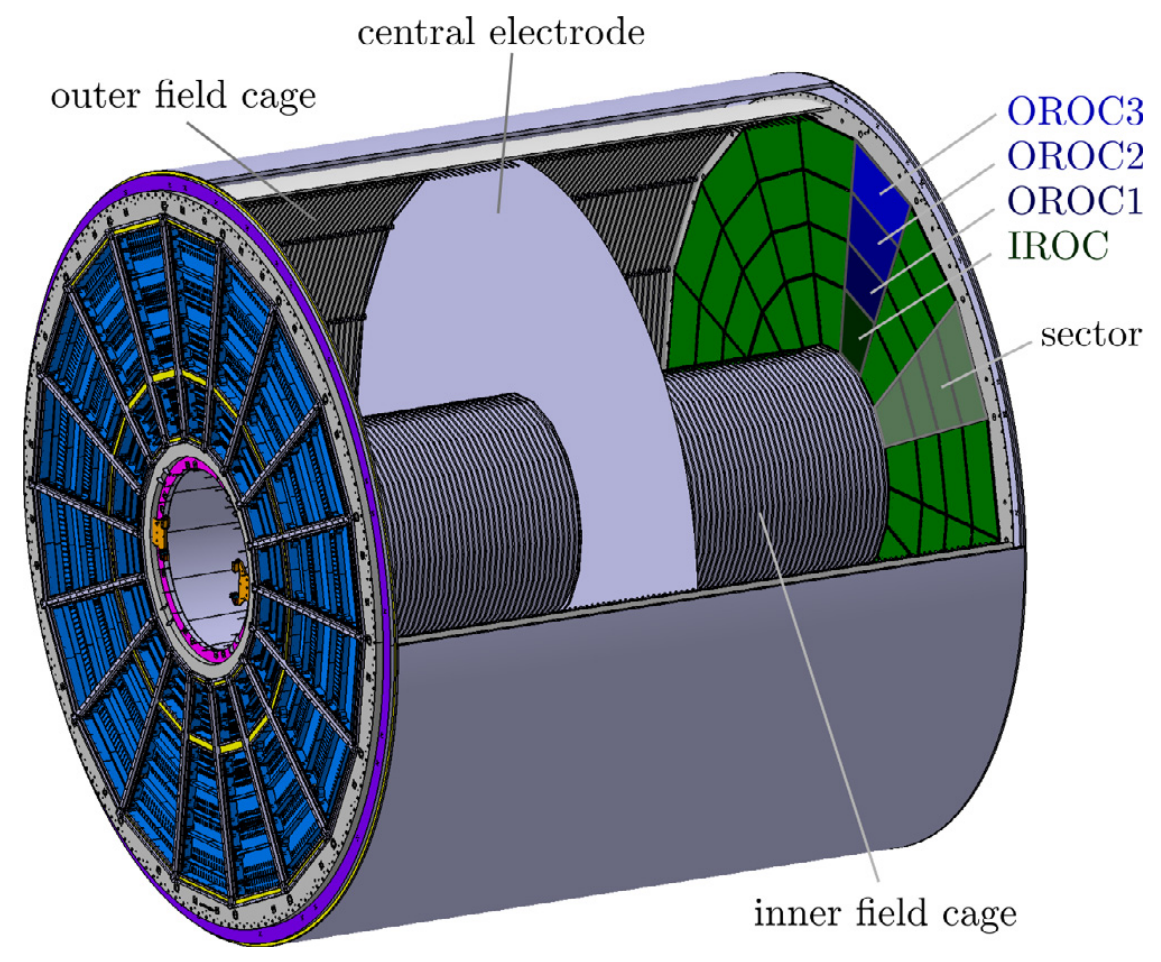
\includegraphics[width=0.65\textwidth]{alice_tpc.png}
				\hfill
				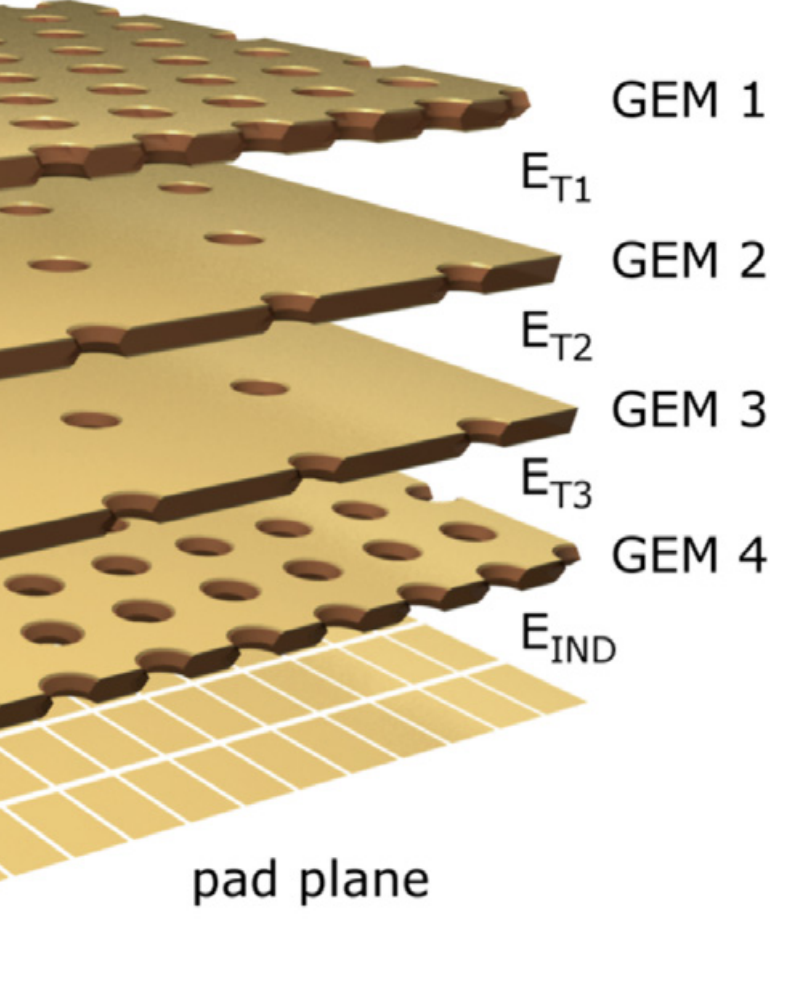
\includegraphics[width=0.33\textwidth]{alice_gem.png}
				\caption{Schematic view of the ALICE \ac{TPC}~\cite{ALICE_upgrade2}. The readout at each endcap is divided into 18 sectors, each subdivided into an Inner Readout Chamber (IROC) with one \ac{GEM} stack and Outer Readout Chamber (OROC) with three \ac{GEM} stacks. A~visualization of a~\ac{GEM} stack is on the right~\cite{ALICE_gem}.}
				\label{fig:alice}
			\end{figure}
			
		\subsection{CERES/NA45 radial-drift TPC}
			In 1998, the CERES/NA45 (Cherenkov Ring Electron Spectrometer) experiment (\cref{fig:ceres}) at the CERN SPS was upgraded with the first \acf{rTPC} to achieve a~higher momentum resolution~\cite{ceres}. Unlike a~standard \ac{TPC}, the electric field \qtyrange{600}{200}{\V\per\cm} was arranged radially with the magnetic field (inhomogeneous, up to \qty{0.5}{\tesla}) by two solenoidal coils with opposite polarity. The outward drift of the ionization electrons is affected by the crossing fields as shown in \cref{eq:drift} and the drift velocity is not uniform due to the varying electric field. The \ac{rTPC} was filled with an 80:20 Ne:CO$_2$ gas mixture, which has relatively small diffusion coefficients and Lorentz angle. The readout was handled by conventional \acp{MWPC} (\cref{fig:ceres_readout}).
			
			\begin{figure}
				\centering
				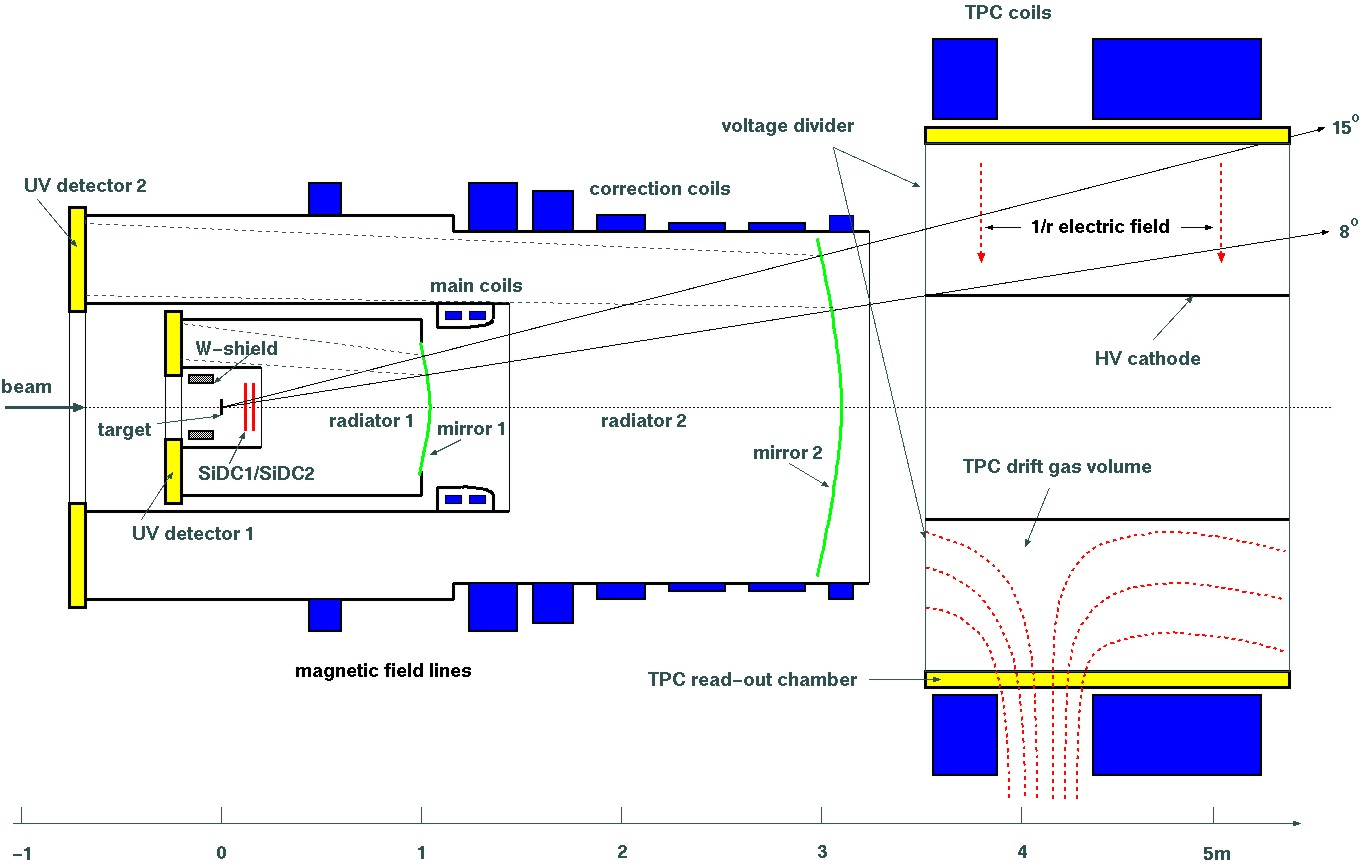
\includegraphics[width = \textwidth]{ceres.jpg}
				\caption{Experimental setup of the CERES/NA45 experiment with two \acfp{RICH} on the left and a~\ac{rTPC} on the right. The magnetic field (red) is generated by two solenoidal coils (blue) with opposite polarity. Produced ionization electrons drift outward radially towards the readout chamber (yellow)~\cite{ceres}.}
				\label{fig:ceres}
			\end{figure}
			\begin{figure}
				\centering
				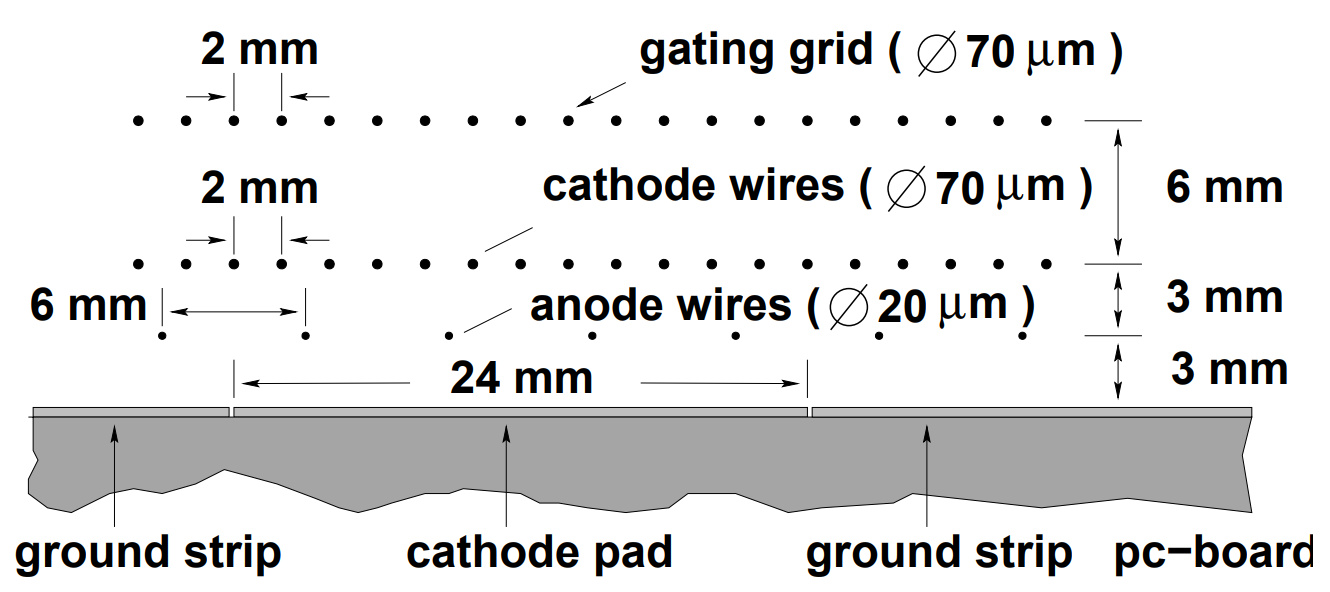
\includegraphics[width=0.7\textwidth]{ceres_readout.png}
				\caption{Cross section of a~CERES/NA45 readout \ac{MWPC}. The wires are stretched in the azimuthal direction above the pad plane. The gating grid controls the passage of electrons and ions.~\cite{ceres}.}
				\label{fig:ceres_readout}
			\end{figure}
			
			The field configuration in an \ac{rTPC} enables a~larger number of pads compared to a~standard \ac{TPC}, leading to improved spatial resolution and possibility of larger multiplicity rates. Since the drift time is lower, the detector is faster.
			
			After an algorithm described in this thesis was developed for our \acp{OFTPC} at \ac{IEAPCTU}, we noticed the similarities with the approach used by the CERES/NA45 \ac{rTPC}, when accounting for the transport process of charged clusters in the complex fields. The detector hit coordinates (pad, time, and plane) were transformed using look\nobreakdash-up tables. The tables were calculated using a~Runge-Kutta method to integrate the Langevin approximation of the drift velocity (\cref{eq:drift}). The drift velocity in the radial field was calibrated using seven parallel laser rays. This calibration was then used to make a~correction compared to the MAGBOLTZ Monte Carlo drift~\cite{magboltz}.\red{~Measured mobility differs significantly from MAGBOLTZ, but this might be improved in the newer versions?} The tracks were fitted using reference tables with hit coordinates of tracks simulated with GEANT Monte Carlo\red{~(not such a big problem for us right now, might be an idea if the reconstruction gets too slow)}.
			
		\subsection{Other interesting radial-drift TPCs}
			\red{muEDM at PSI: \url{https://arxiv.org/pdf/2307.01535},\\ FTPC at STAR at RHIC: \url{https://arxiv.org/pdf/nucl-ex/0211014}}
			\subsubsection{BONuS12 rTPC}
				In 2020, the \acf{BONuS12} experiment used an \ac{rTPC} (\cref{fig:bonus}) to measure low-momentum spectator protons produced in $e^- d \rightarrow e^- p_\text{s}X$ scattering~\cite{bonus}. It was filled with a~80:20 He:CO$_2$ gas mixture and placed inside a~\qty{4}{\tesla} solenoidal magnetic field, perpendicular to the radial electric field (\qty{1100}{\V\per\cm} on average), tilting the drift (see \cref{eq:lorentz}). The amplification used cylindrical triple \ac{GEM} stacks.
				
				\begin{figure}
					\centering
					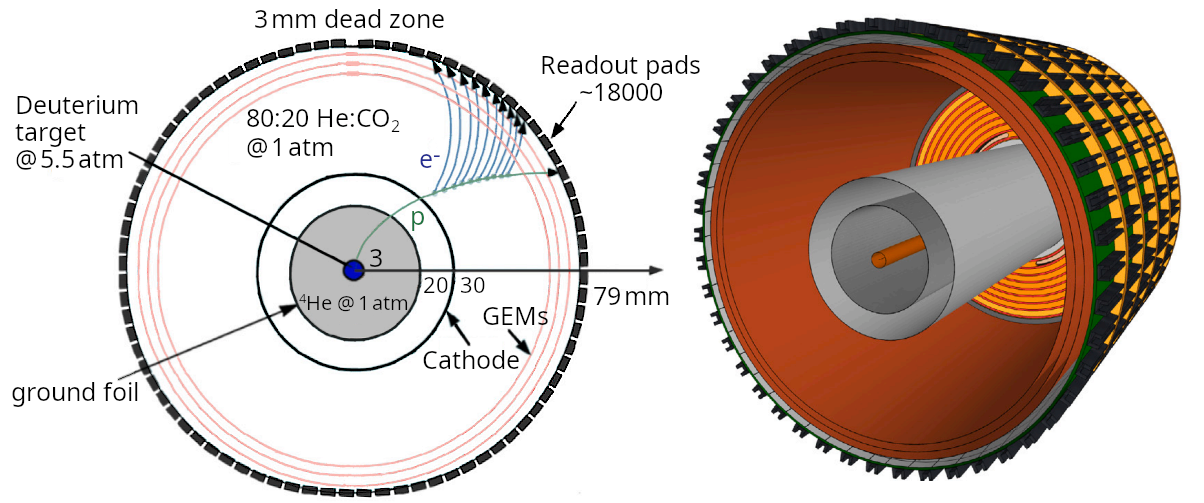
\includegraphics[width=\textwidth]{bonus12_edit.png}
					\caption{Schematic view of the \ac{BONuS12} \ac{rTPC}~\cite{bonus}.}
					\label{fig:bonus}
				\end{figure}
				
				\garfieldpp simulations and study of reconstructed tracks have shown that the radial component of the drift velocity almost proportional to the radial electric field, and the $r$\nobreakdash-coordinate can be reconstructed using an analytical formula. Similarly, the azimuthal component is nearly proportional to the radial component, resulting in a~largely constant Lorentz angle between the radial and actual direction, and the $\phi$\nobreakdash-coordinate can be solved analytically. The remaining $z$\nobreakdash-coordinate stays undistorted. The momentum is determined by fitting tracks with a~helix, while accounting for the energy losses (the small variability of magnetic field along the $z$\nobreakdash-axis has a~negligible effect).
				
			\subsubsection{ALPHA-g rTPC}
				In 2023, the \acf{ALPHA} collaboration published results of measurements of antihydrogen~(\antiH) annihilation\footnote{The main \antip annihilation mode is into several $\pi^\pm$ and $\pi^0$, only the $\pi^\pm$ tracks are long enough to be reconstructed. The scattering of $\pi^\pm$ is not negligible, and photons from $\pi^0$ decay create $e^+e^-$ pairs as background.} after release from magnetic confinement, showing that it behaves in a~way consistent with gravitational attraction to the Earth~\cite{alpha_nature}. They used a~\qty{2.3}{m} long \ac{rTPC} (\cref{fig:alpha-g}) with a~\qty{40}{cm} outer and \qty{20}{cm} inner diameter in a~\qty{1}{\tesla} solenoidal magnetic field, and filled with an Ar/CO$_2$ mixture~\cite{alpha_rtpc}. The readout consists of an \ac{MWPC} (\cref{fig:alpha-g_drift}). The radial confinement of the cold~\antiH is achieved with a~superconducting octupole magnet, the axial with a~set of so\nobreakdash-called \emph{mirror} coils.
				
				\begin{figure}
					\centering
					\begin{subfigure}[t]{0.49\textwidth}
						\centering
						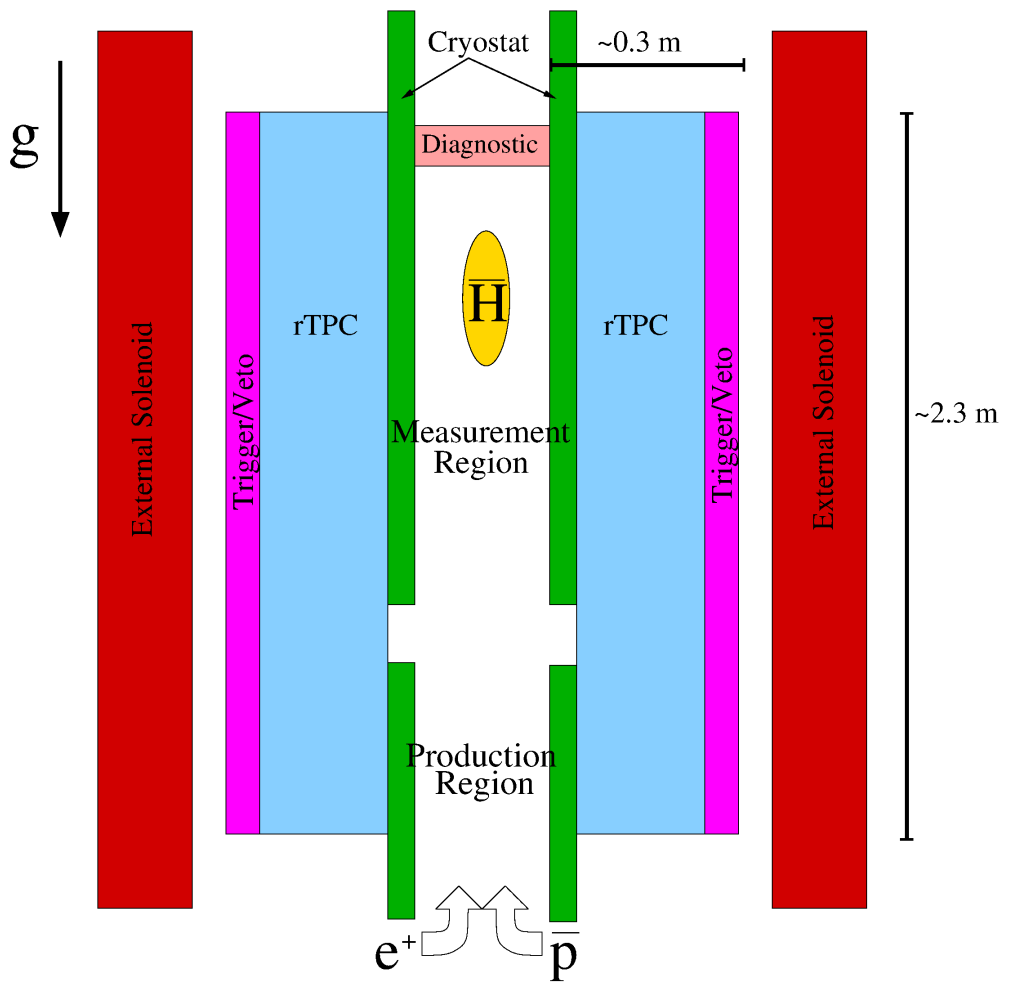
\includegraphics[width=\textwidth]{alpha-g.png}
						\caption{Sketch of \acs{ALPHA}\protect\nobreakdash-g. Antiprotons and positrons are injected from the bottom and form~\antiH in a~Penning trap while being cooled by the cryostat (green). The annihilation is reconstructed by the \ac{rTPC} (blue).}
						\label{fig:alpha-g}
					\end{subfigure}
					\hfill
					\begin{subfigure}[t]{0.49\textwidth}
						\centering
						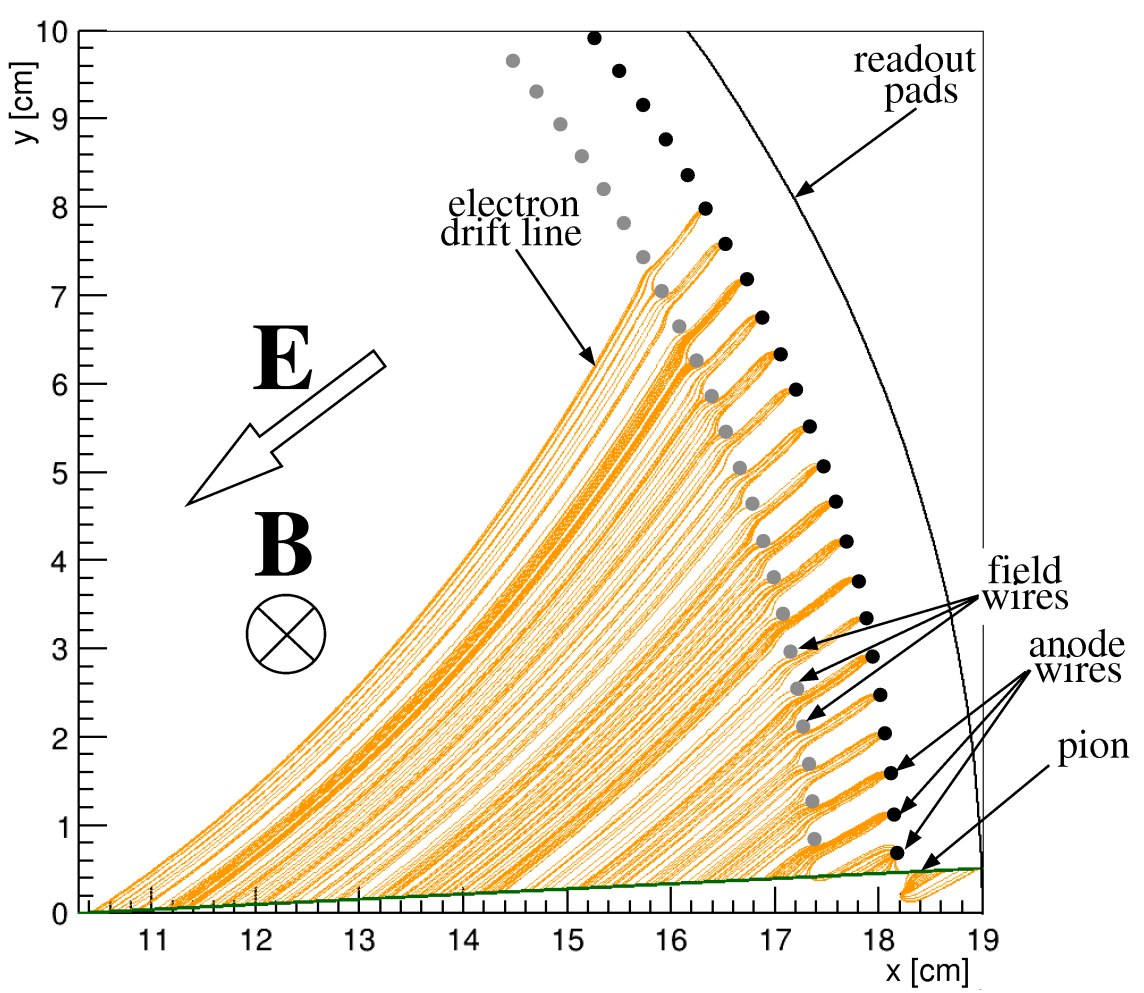
\includegraphics[width=\textwidth]{alpha-g_drift.png}
						\caption{Cross section view of the \ac{rTPC} (\garfieldpp simulation). The electrons (orange) produced by a~pion track (green) drift towards the anode wires, while influenced by the axial magnetic field. The size of the field and anode wires is exaggerated.}
						\label{fig:alpha-g_drift}
					\end{subfigure}
					\caption{Schematic view of the \acs{ALPHA}\protect\nobreakdash-g detector~\cite{alpha_rtpc}.}
				\end{figure}
				
				The $r$\nobreakdash-coordinate of the ionization cluster is reconstructed from the drift time using a~tabulated space-time relation. The 3D position of the interaction (cluster) vertex is obtained by matching the wires and pads by drift time using a k\nobreakdash-d tree algorithm. Reconstructed tracks are fitted with a~helix using the least squares method~\cite{alpha_reco}.
	
	\section{Readout}
	\label{sec:readout}
		\subsection{Multi-Wire Proportional Chamber}
		\label{sec:MWPC}
			In most \acp{TPC} operated in experiments, \acf{MWPC} was used for the readout (\cref{fig:mwpc}). The electrons enter the chamber through a~cathode grid and get accelerated by a~strong electric field towards the parallel, thin anode wires and create an avalanche, multiplying the signal. The trajectory can be reconstructed from the drift time and two coordinates measured using
			\begin{enumerate}[nosep,label=\alph*)]
				\item two segmented cathodes (wires or strips) rotated by $\ang{90}$ or
				\item the ratio of charge collected on two sides of the hit resistive wires.
			\end{enumerate}
			For high counting rates, the positive ions from the avalanches accumulate, creating a~space charge that distorts the electric field. This can be solved by using a~gating grid near the readout plane to collect these ions at the cost of introducing a~dead time in the detector.
			
			\begin{figure}
				\centering
				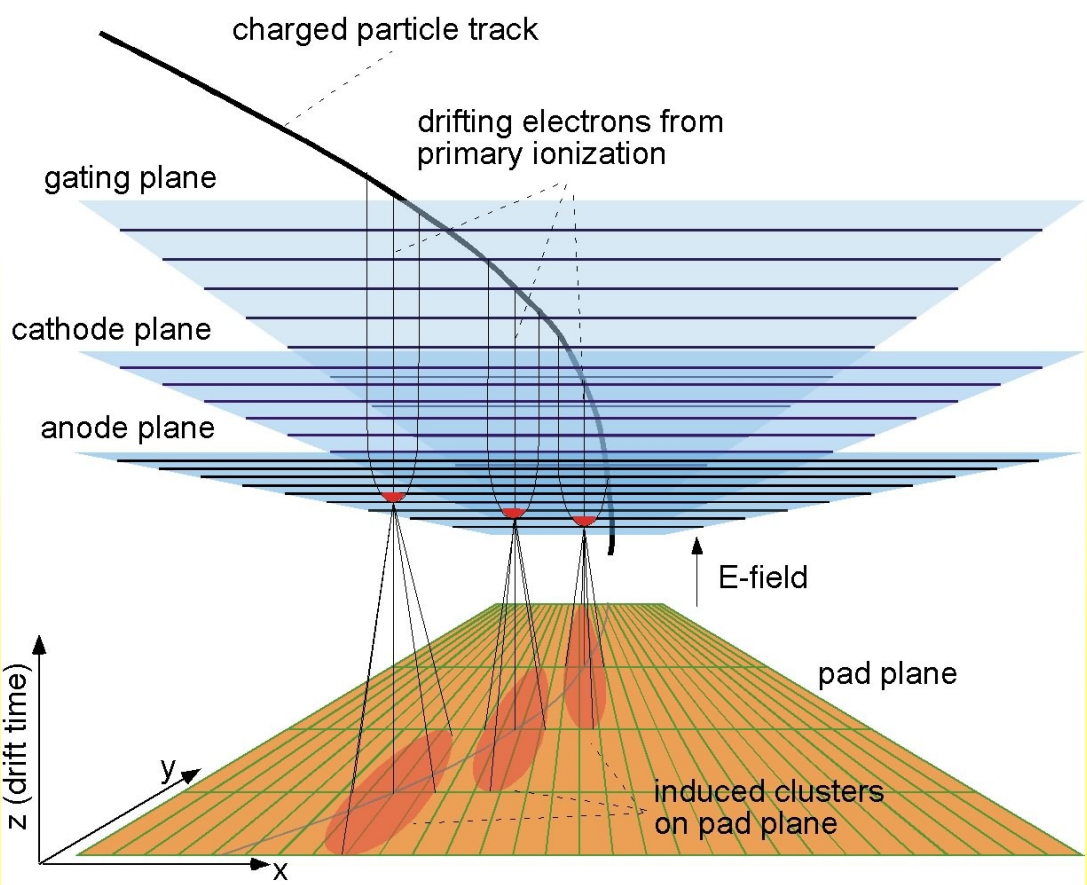
\includegraphics[width=0.7\textwidth]{mwpc.png}
				\caption{Schematic view of the ALICE \ac{MWPC} readout (working principle)~\cite{mwpc}.}
				\label{fig:mwpc}
			\end{figure}
			
		\subsection{Micro-Pattern Gaseous Detectors}
		\label{sec:mpgd}
			In order to avoid \ac{MWPC} limitations (e.g., diffusion, wire $\mathbf{E}\cross\mathbf{B}$ effect, space charge effects), a~family of \acf{MPGD} technologies are being developed. The readouts can reach higher spatial resolution (down to $\qty{30}{\um}$) with faster response time ($\unit{\ns}$ range) and much higher rate capability.
			
			\subsubsection{Gas Electron Multiplier}
				A~\acf{GEM} is a~thin metal-coated polyimide sheet with a~dense pattern of small, chemically etched holes (\cref{fig:gem}). The amplification is achieved by applying voltage across the metal layers and placing the foil between two moderate uniform electric fields. This creates a~strong electric field inside the holes that accelerates the incoming electrons and causes avalanches (see \cref{fig:gemsim}). Some charges may land on the dielectric surfaces due to diffusion, modifying the field and affecting gain.
				
				\begin{figure}
					\centering
					\begin{subfigure}[t]{0.48\textwidth}
						\centering
						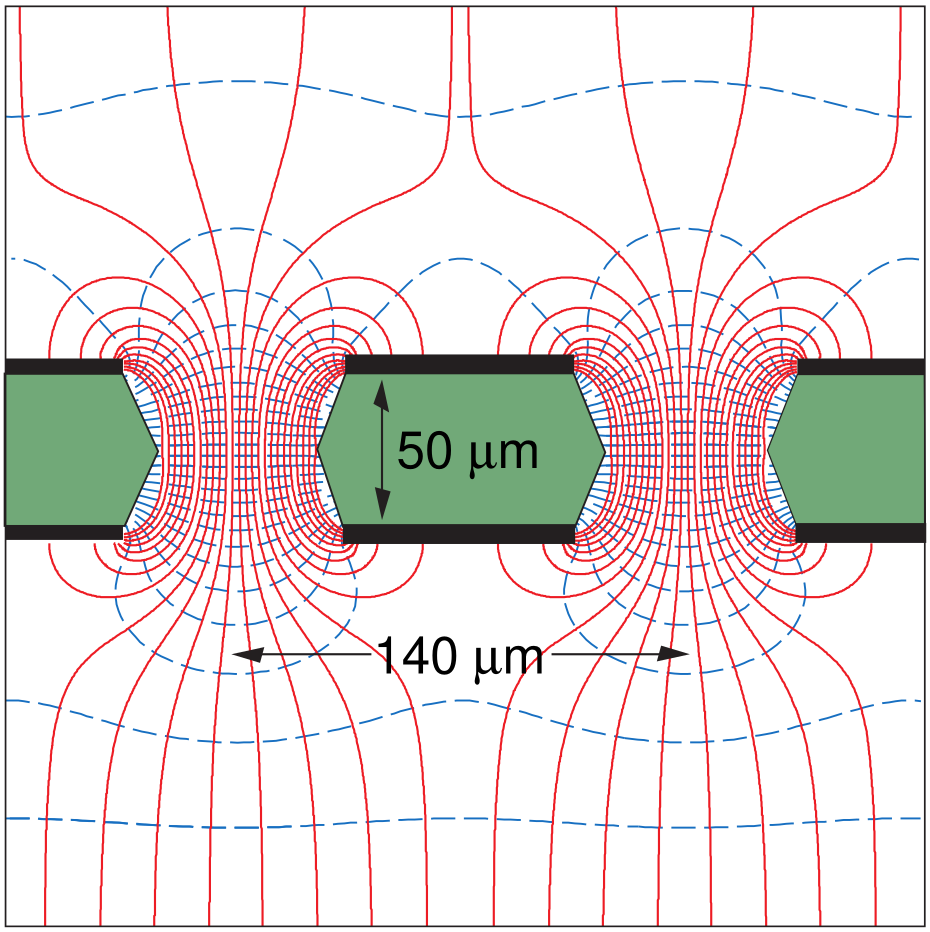
\includegraphics[width=\textwidth]{gem_schem.png}
						\caption{A~schematic view of a~\ac{GEM} cell with its typical dimensions, electric field lines (red), and equipotentials (blue)~\cite{pdg2024}.}
						\label{fig:gem_schem}
					\end{subfigure}
					\hfill
					\begin{subfigure}[t]{0.48\textwidth}
						\centering
						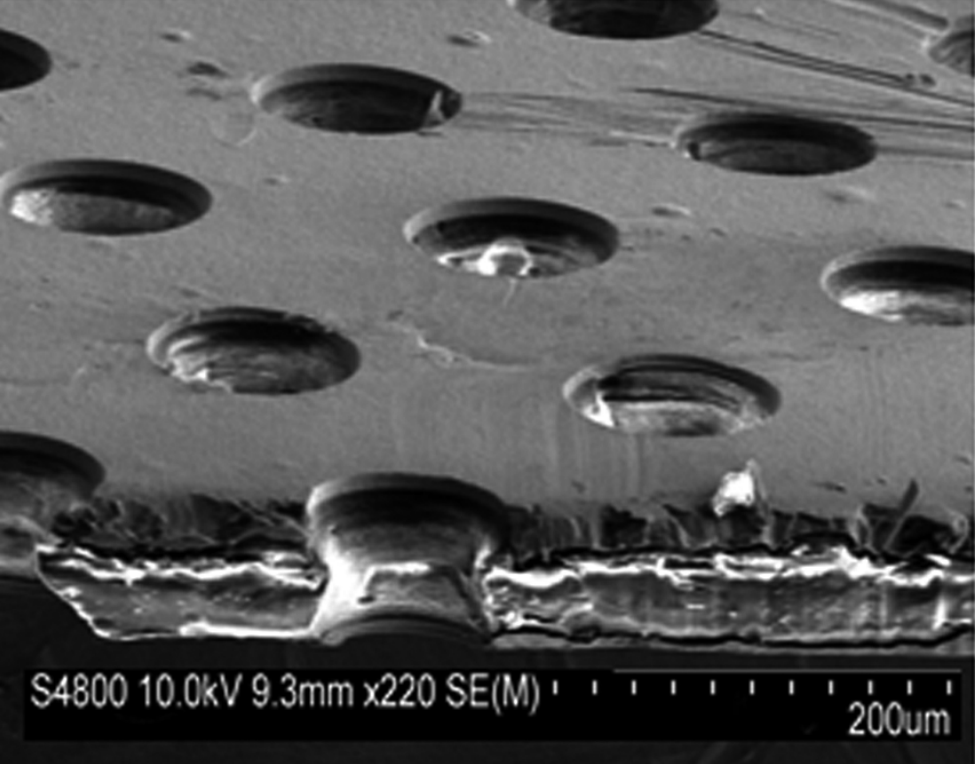
\includegraphics[width=\textwidth]{gem_hole.png}
						\caption{A~scanning electron microscope image of a~\ac{GEM} foil~\cite{gemhole}.}
						\label{fig:gemhole}
					\end{subfigure}
					\caption{\acf{GEM}.}
					\label{fig:gem}
				\end{figure}
				\begin{figure}
					\centering
					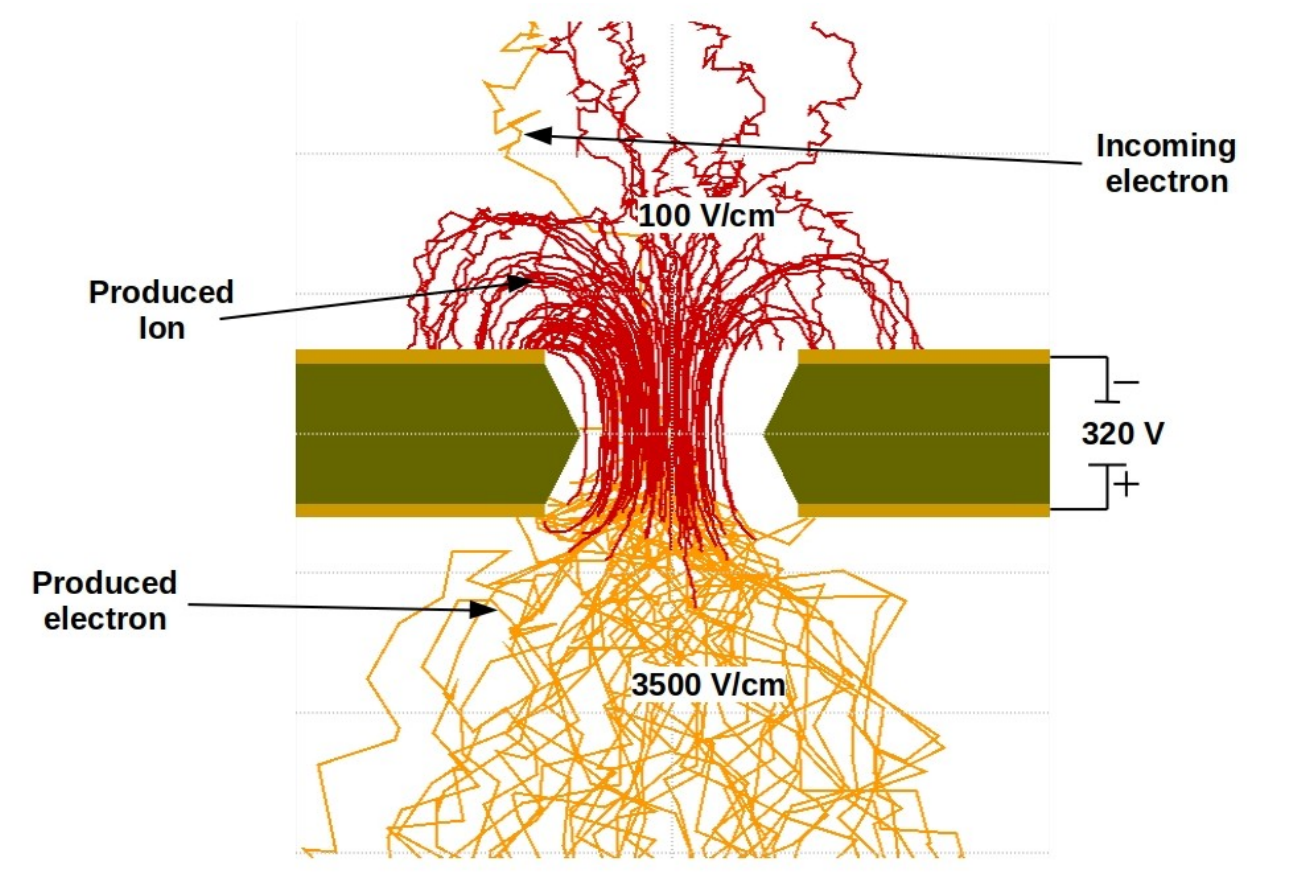
\includegraphics[width=0.8\textwidth]{gemsim.png}
					\caption{Garfield simulation of an avalanche in a \ac{GEM} hole~\cite{gemsim}. An incoming electron (orange) is accelerated in the strong electric field of the \ac{GEM} and causes further ionization multiplying the number of free electrons (orange). Most of the produced cations (red) are captured by the \ac{GEM} cathode.}
					\label{fig:gemsim}
				\end{figure}
				
				Double or triple stacks of \acp{GEM} are usually used to create a~sufficient gain while maintaining stability (reducing discharges). From the last foil, the electrons drift to a~segmented anode where the signal is read. The ion backflow is reduced compared to \ac{MWPC}.
				
				A~cheaper alternative (especially for large area coverage) is a~\ac{THGEM} with a~\textapprox10\nobreakdash-fold upscaling of geometrical parameters. It can be made by mechanically drilling holes into a~standard \ac{PCB} and creating a~circular rim around the holes by etching the metal coating.
			
			\subsubsection{Micromegas}
				In a~\ac{Micromegas}\orange{~(in sources I viewed it is not capitalized)} electrons pass through a~fine mesh (made out of very thin wires) into a~narrow amplification gap where they are multiplied in the high field and read as a~signal on the segmented anode (\cref{fig:micromegas_schem}). Very high field (\qtyrange{30}{80}{\kV\per\cm\squared}) is necessary to achieve sufficient gain. Ion backflow is heavily suppressed by the mesh. 
				
				A~Timepix chip (a~high granularity pixel detector) can be used for the readout anode to achieve the best spatial resolution, making an integrated readout called GridPix (\cref{fig:micromegas_sem}). Thanks to the high spatial resolution, it is possible to distinguish individual electron clusters, which enables a~new method of particle identification.
				
				\begin{figure}
					\centering
					\begin{subfigure}[t]{0.54\textwidth}
						\centering
						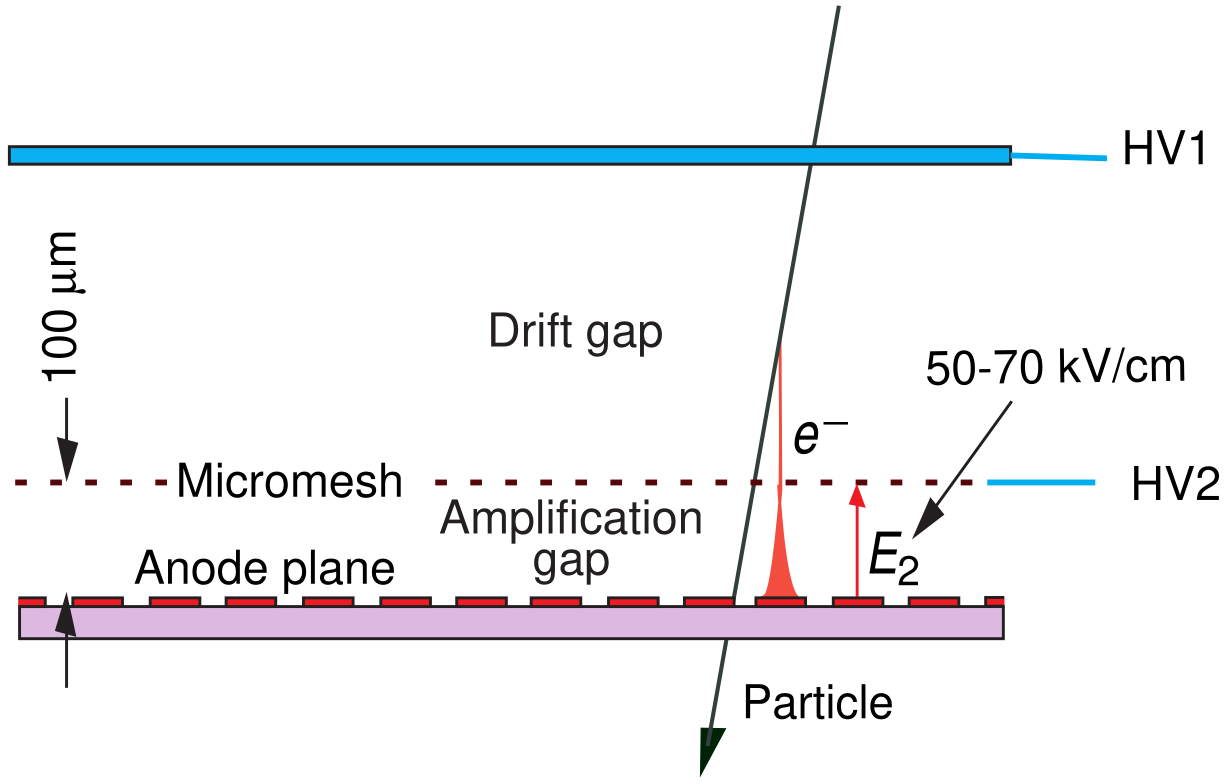
\includegraphics[width=\textwidth]{micromegas_schem.png}
						\caption{A~schematic view of a~\ac{Micromegas} detector.}
						\label{fig:micromegas_schem}
					\end{subfigure}
					\hfill
					\begin{subfigure}[t]{0.44\textwidth}
						\centering
						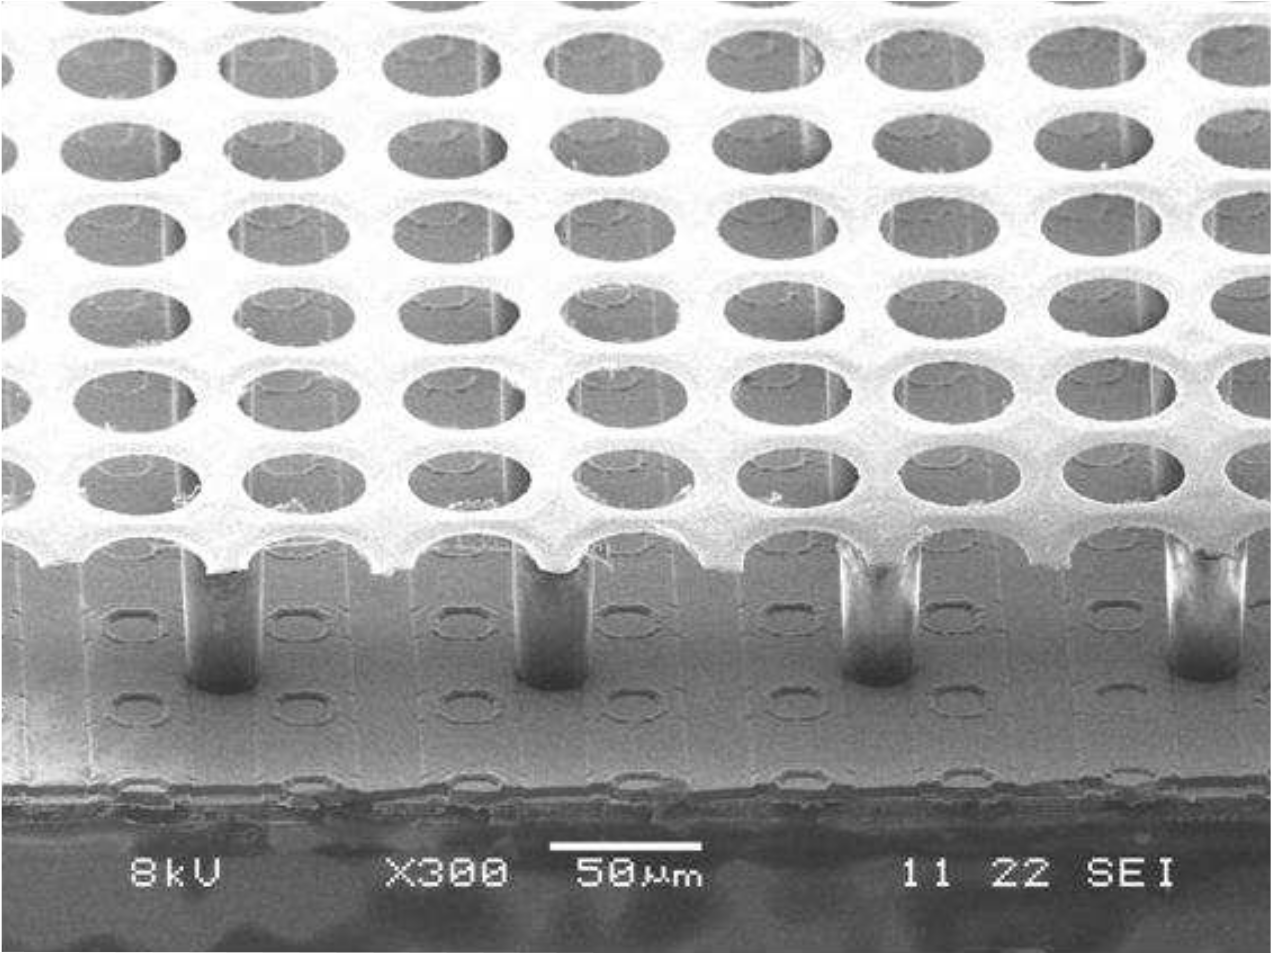
\includegraphics[width=\textwidth]{micromegas_sem.png}
						\caption{A~scanning electron microscope image of a~\ac{Micromegas} "GridPix" detector.}
						\label{fig:micromegas_sem}
					\end{subfigure}
					\caption{\acf{Micromegas}~\cite{pdg2024}.}
					\label{fig:micromegas}
				\end{figure}
			
			\subsubsection{Other MPGDs}
				A~\ac{RPWELL} consists of a~\ac{THGEM} with only the top side metal-coated, mounted on a~resistive film deposited on a~thin isolating sheet (which is read out similarly to a~\ac{RPC}). Due to the higher field in the closed holes of the \ac{THGEM}, a~higher gain can be reached for the same voltage. A~\ac{uRWELL} is a~similar architecture with \textapprox7~times smaller pitch (distance between holes). These options provide a~better spark resistance and could allow to cover large areas for a~lower cost.
				
				A~\ac{uPIC} is a~\ac{PCB} with anode strips on one side and orthogonal cathode strips on the other. The cathode has a~resistive coating and a~regular pattern of uncoated regions with anode "dots" penetrating the \ac{PCB} at the centers.
	
	\section{Orthogonal Fields TPC at IEAP CTU}
	\label{sec:oftpc}
		At \ac{IEAPCTU}, we are going to use six identical atypical \acp{TPC} with inhomogeneous toroidal magnetic field \textbf{orthogonal} to the electric field\orange{~(details below)}, hereafter referred to as \acf{OFTPC}. It has the shape of isosceles trapezoidal prism 16~centimeters high with triple\nobreakdash-\ac{GEM} readout on one of its bases. Dimensions of the \ac{OFTPC} are discussed in detail in section~\ref{sec:coor} below. Throughout this thesis, we assume a~uniform electric field along the $z$~axis with $E_z = -400$~V/cm.\red{~Isn't the field affected by the \acp{MWPC}? Eventually a simulation will be needed.} Measured particles enter the \ac{OFTPC} through a~window after crossing the \ac{MWPC}.\red{~Gas mixture used in the detector (70/30) and its effect -- some graph with the mixture, reasons for the choice. Add a~figure of the real TPC. More about the design choices.}
		
		
		\subsection{Motivation and Associated Challenges}
			The reasons for the unusual field layout are mostly cost related:
				\begin{enumerate}[nosep,label=\alph*)]
					\item we use permanent magnets instead of a~solenoid and parallel fields are difficult to accomplish this way,
					\item granularity of the \ac{TPC} readout is limited in order to fit one SAMPA/SRS hybrid in each sector -- parallel fields would bend the trajectories parallel to the readout requiring more pads and different architecture.
				\end{enumerate}
			In this thesis, we will show that such a~setup can reach a~similar energy resolution as common cylindrical \acp{TPC} while reducing the overall cost.
			
			The layout introduces two complications to the track reconstruction -- the trajectory in inhomogeneous field is not circular and the drift is distorted by the magnetic field as shown in the Equation~\ref{eq:drift}(in our case $\omega\tau \approx 0.08$\red{~for 0.3~T assuming $\mu\approx0.25$~T$^{-1}$, varies inside the detector}). We will deal with these effects in the upcoming chapters.
			
			The diffusion in such setup is larger since parallel orientation reduces diffusion by curling the electrons in the $x$\nobreakdash-$y$ direction (see Equation~\ref{eq:difmag}), but for our relatively weak magnetic field and short drift distance, the difference is negligible.
	
		\subsection{Coordinate Systems and Dimensions}
		\label{sec:coor}
			In order to describe events in our detector, we use three distinct spaces: the detector space $\mathcal{D}$, the readout space $\mathcal{R}$ and the pad space $\mathcal{P}$\orange{~(different spaces that describe different things and each has their own coordinate system, so maybe rename the section somehow?)}. Each space is later used to represent ionization electrons at different stages of the detection process: their creation in the gas, their final position when hitting the readout plane, and finally their representation in the discrete pad space.
		
			\subsubsection{Detector Space}
				The detector space $\mathcal{D}$ represents the physical space of our detector. We describe it using Cartesian coordinates $(x,y,z)$. The $z$-axis is the detector's axis of symmetry, with its negative direction aligned with the proton beam. The origin $(0,0,0)$ is located at the center of the irradiated target. The positive $x$\nobreakdash-axis passes through the center of one the \acp{OFTPC} along the intersection of its two planes of symmetry. The $y$\nobreakdash-axis is then chosen to maintain a~right-handed coordinate system.
				
				Since the detector has a~hexagonal symmetry, we use only one of its sectors in this work -- the first sector $\mathcal{D}_1 \subset \mathcal{D}$ which is defined by the condition:
					\begin{equation}
						(x,y,z) \in \mathcal{D}_1 \Leftrightarrow |y| \leq x\tan \frac{\pi}{6}.
					\end{equation}
				Simulations in this sector can be applied to all sectors by rotating the coordinates accordingly. The volume of the \ac{OFTPC} in this sector, which has the shape of a~trapezoidal prism, has these boundaries:
					\begin{linenomath}
						\begin{align}
							x \in [x_\text{min},x_\text{max}] &= [6.51, 14.61] \;\text{cm},\\
							z \in [z_\text{min},z_\text{max}] &= [-8,8] \;\text{cm},\\
							y_\text{max}(x_\text{min}) = -y_\text{min}(x_\text{min}) &=  2.75\;\text{cm},\\
							y_\text{max}(x_\text{max}) = -y_\text{min}(x_\text{max}) &=  7.45\;\text{cm},
						\end{align}
					\end{linenomath}
				where $y_\text{max}(x)$ is the maximal value of the $y$-coordinate for a~given $x$. The readout is located at $z = 8$~cm; for some purposes, we also define the distance to the readout $d_r = 8\;\text{cm}-z$ as an alternative to the $z$-coordinate.\orange{~Keeping this paragraph as it is because the \ac{OFTPC} volume is distinct from the first sector and some parts of this thesis use the space beyond this volume.} The \ac{OFTPC} window has width 3.8~cm and height 4.0~cm.
				
				We also use spherical coordinates $(r,\theta,\varphi)$ with the elevation angle~$\theta$ measured relative to the $xy$ plane. Angles~$\theta$ and~$\varphi$ are useful when describing the direction of $e^+/e^-$~tracks. Their maximal values considered for the initial direction in simulations are $\theta_\text{max} \approx 17.1^\circ$ and $\varphi_\text{max} \approx 16.3^\circ$ as shown in \cref{fig:oftpc}.
				
				\begin{figure}
					\centering
					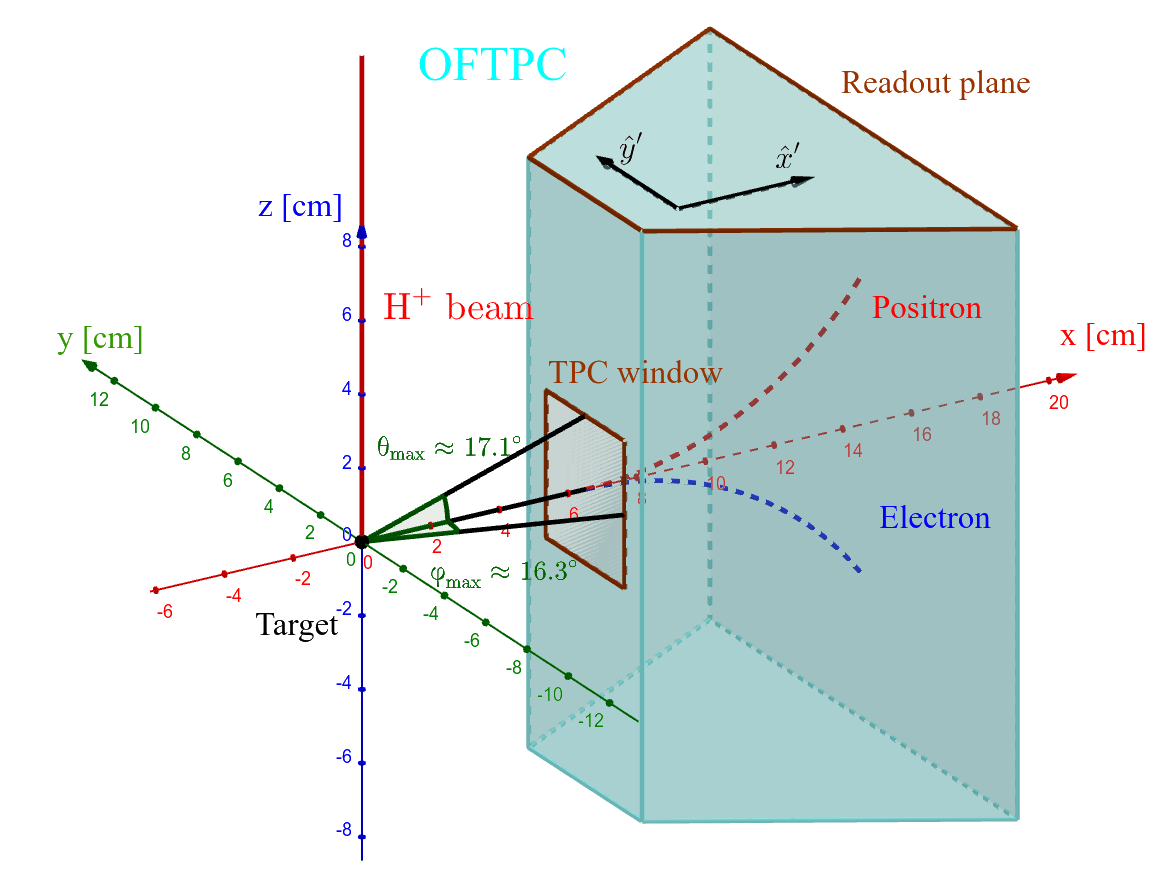
\includegraphics[width=0.8\textwidth]{tpc_ggb.png}
					\caption{Schematics of the first sector \ac{OFTPC} with detector space coordinates.}
					\label{fig:oftpc}
				\end{figure}
			
			\subsubsection{Readout Space}
				The readout space $\mathcal{R}$ represents the drift time and final positions of ionization electrons as measured by an ideal continuous readout. We describe it using coordinates $(x',y',t)$, where $x'$ and $y'$ correspond to the detector coordinates at the readout plane ($z = 8$~cm).
				
				\red{Currently not entirely sure how to put this into a~figure since only $x'$ and $y'$ correspond to the detector coordinates, \textbf{it will make more sense when visualizing the map}. The drift time~$t$ is approximately proportional to~$d_r$.}
			
			\subsubsection{Pad Space}
				The pad space $\mathcal{P}$ represents the time bin and pad number of ionization electrons as measured by an ideal discrete readout:
					\begin{equation}
						\mathcal{P} = \{(n_\text{pad},n_t)\in\mathbb{N}^2 \mid n_\text{pad}\leq128\}.
					\end{equation}
				\red{\textbf{Rewrite to reflect this:} Technically both values can be zero as defined in the code (max channel 127). It is not really a~subspace of $\mathcal{R}$ but there is a mapping from $\mathcal{R}$ to $\mathcal{P}$. It is a discretization of a~part of $\mathcal{R}$, the mapping can be adjusted depending on the simulation. If we assume uniform electric field there will be gaps, we don't use gaps in the reconstruction since the electrons should be pulled towards the pads.}
				
				The readout of the \ac{OFTPC} will consist\red{~(is the design final?)} of 128~rectangular pads arranged in a~staggered pattern. Parameters of the pad layout are shown in \cref{fig:padlayout}. The bottom left corner of $n$\nobreakdash-th pad has coordinates $(x_{1,n},y_{1,n})$, the  top right $(x_{2,n},y_{2,n})$ and its center has coordinates $(x_{c,n},y_{c,n})$. The gap between neighboring pads is $g=0.08$~cm. Time will be read out in discrete bins of size $t_\text{bin}=100$~ns\red{~(details?)}.\red{~Could also describe pad-related functions.}
			
				\begin{figure}[H]
					\centering
					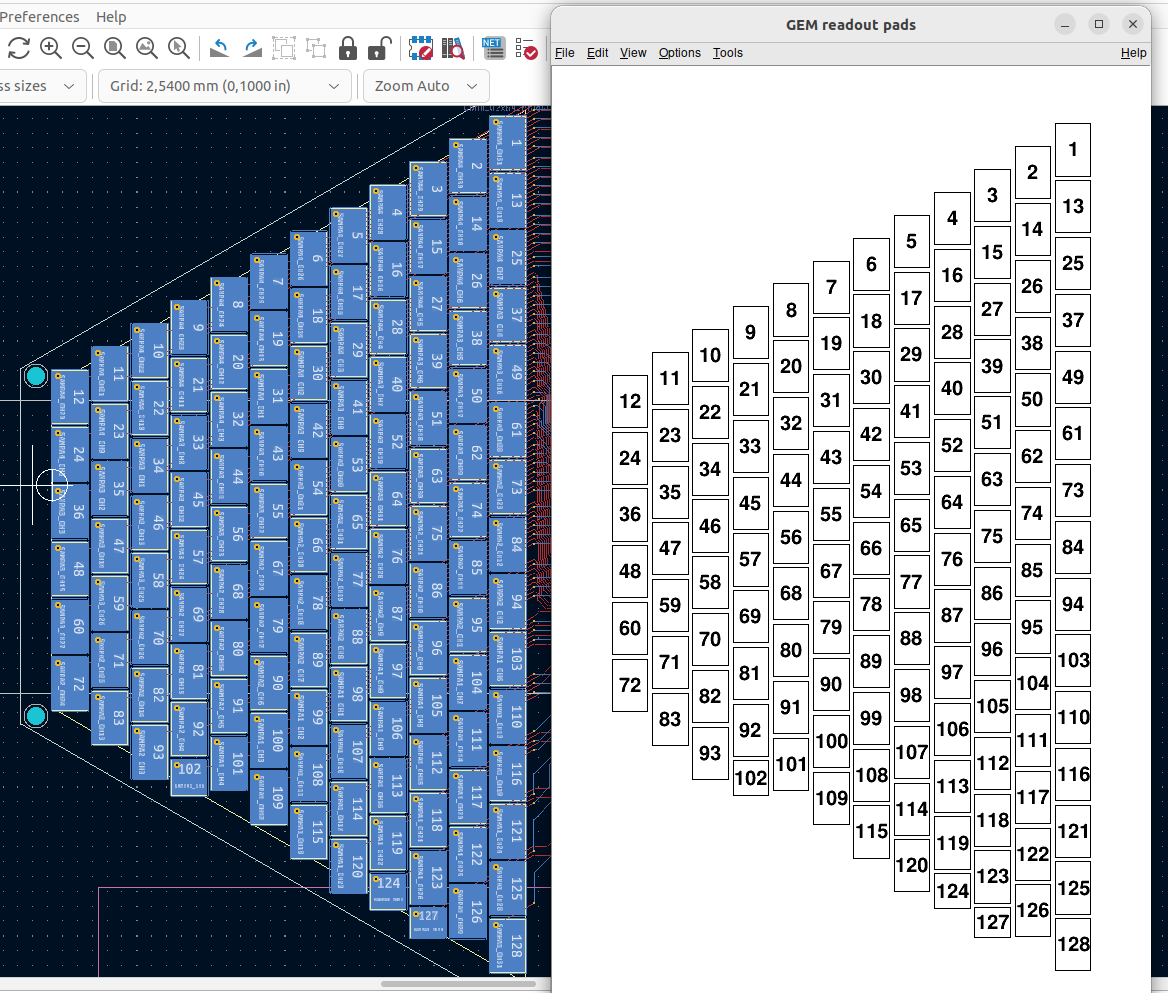
\includegraphics[width=\textwidth]{padlayout.png}
					\caption{Pad layout of the \ac{OFTPC} and its parameters. Pads 102, 124 and 127 are irregular, the rest has the same dimensions.}
					\label{fig:padlayout}
				\end{figure}
		
		\subsection{Magnetic Field Simulation}
		\label{sec:mag}
			The magnetic field inside our detector is produced by six permanent magnets. It was simulated using Ansys Maxwell\red{~(citation)} which gives us values on a~regular grid.\red{~More details, vacuum tube, magnets (homogeneous?, density?).} Visualization of the magnetic field is shown in \cref{fig:mag}. Whenever we need to work with values outside this grid, we use trilinear interpolation described below.
			
			\begin{figure}
				\centering
				\begin{subfigure}[t]{0.45\textwidth}
					\centering
					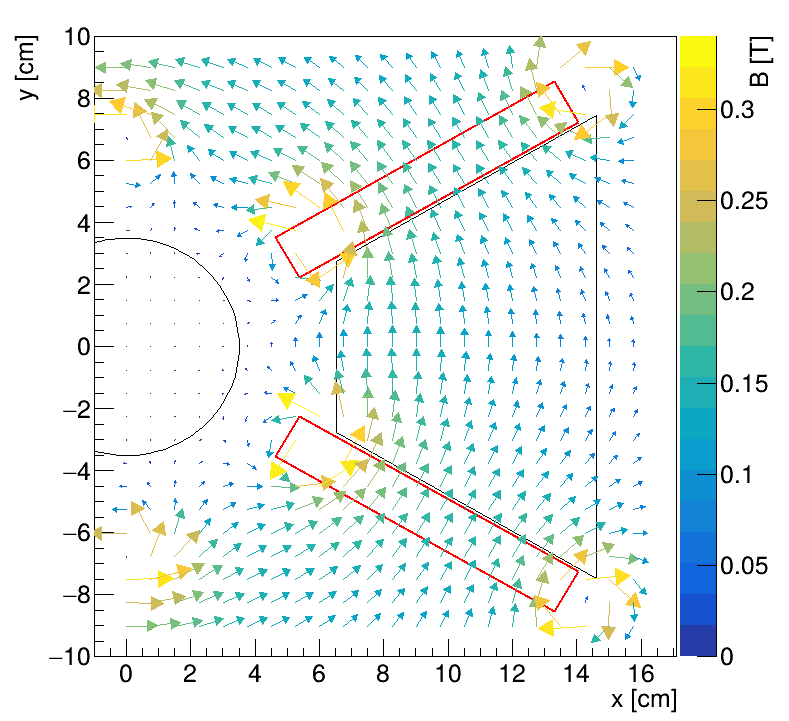
\includegraphics[width=\textwidth]{mag_xy.png}
					\caption{Field in the $xy$ plane.}
				\end{subfigure}
				\hfill
				\begin{subfigure}[t]{0.45\textwidth}
					\centering
					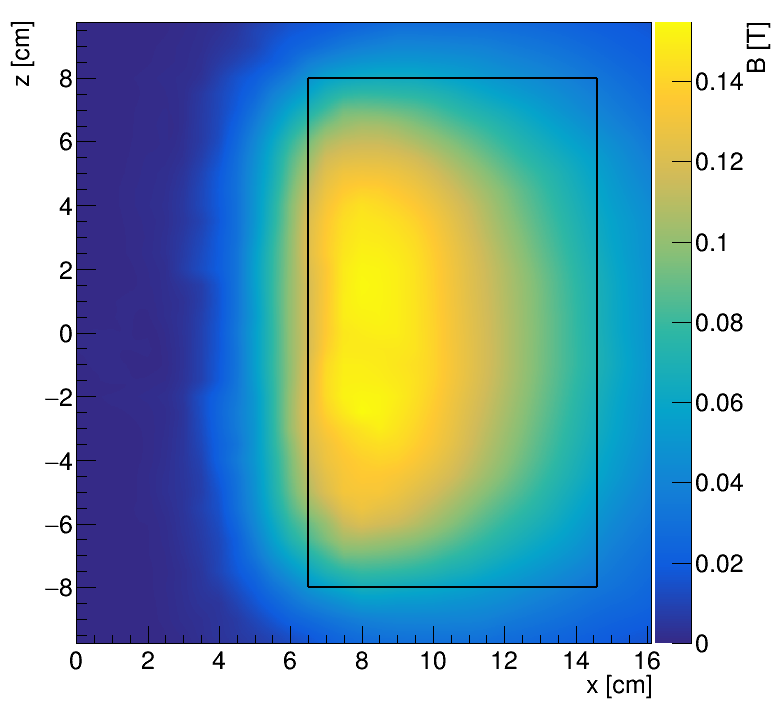
\includegraphics[width=\textwidth]{mag_xz.png}
					\caption{Field magnitude in the $xz$ plane.}
				\end{subfigure}
				\caption{Magnetic field simulation results. The \ac{OFTPC} volume and the vacuum tube are marked with black lines, the magnets are marked with red lines.\red{~The coordinates of the magnets from the CAD drawing seem to be 9/10 of the ones from the magnetic simulation (fixed, the magnetic simulation parameters are off).}}
				\label{fig:mag}
			\end{figure}
		
			\subsubsection{Trilinear Interpolation}
			\label{sec:trilin}
				Trilinear interpolation is a~3D generalization of linear interpolation\footnote{Linear interpolation in point $x\in(x_1,x_2)$ of a~function $f\colon\mathbb{R}\to\mathbb{R}$ known in points $x_1 < x_2$ is the convex combination $\widehat{f}(x) = (1-x_d)f(x_1)+x_d f(x_2)$, where $x_d = \frac{x-x_1}{x_2-x_1} \in (0,1)$.}. It can be used to interpolate a~function whose values are known on a~regular grid with rectangular prism cells. We use this simple method for interpolating the magnetic field, and it is later used in Section~\ref{sec:grad} to interpolate the Ionization Electron Map, a~key component of our track reconstruction algorithm. In both cases, we use a~regular cubic grid\red{~(apparently it is also called a~Cartesian grid)}.
				
				Let us consider a~cell of our regular grid (a~cube) with an edge of length~$a$ containing the point $\mathbf{C} = (x,y,z)$ where we want to interpolate a~function $f\colon\mathbb{R}^3\to\mathbb{R}$. We know the values of this function at the vertices of the cell $\mathbf{C}_{ijk} = (x_0+ia,y_0+ja,z_0+ka)$, where $\mathbf{C}_{000} = (x_0,y_0,z_0)$ is the origin of the cell\orange{~(is that clear?)}, and $i,j,k \in \{0,1\}$ are indices. We also define the points $\mathbf{C}_{ij} = (x,y_0+ia,z_0+ja)$ and $\mathbf{C}_i=(x,y,z_0+ia)$. Then the interpolated value $\widehat{f}(\mathbf{C})$ can be calculated as a~composition of three linear interpolations (see \cref{fig:trilin}):
					\begin{alignat}{3}
						\label{eq:linterpol}
						\widehat{f}(\mathbf{C}_{ij}) &= (1-x_d)\,f(\mathbf{C}_{0ij}) \,&+&\,x_d\, f(\mathbf{C}_{1ij}),\\
						\label{eq:linterpol2}
						\widehat{f}(\mathbf{C}_{i}) &= (1-y_d)\,\widehat{f}(\mathbf{C}_{0i}) &+&\,y_d\, \widehat{f}(\mathbf{C}_{1i}),\\
						\label{eq:linterpol3}
						\widehat{f}(\mathbf{C}) &= (1-z_d)\,\widehat{f}(\mathbf{C}_0) &+&\,z_d\, \widehat{f}(\mathbf{C}_1),
					\end{alignat}
				where $x_d$, $y_d$, and $z_d$ are given as follows:
					\begin{equation}
						x_d = \frac{x-x_0}{a},~y_d = \frac{y-y_0}{a},~z_d = \frac{z-z_0}{a}.
					\end{equation}
					
				\begin{figure}
					\centering
					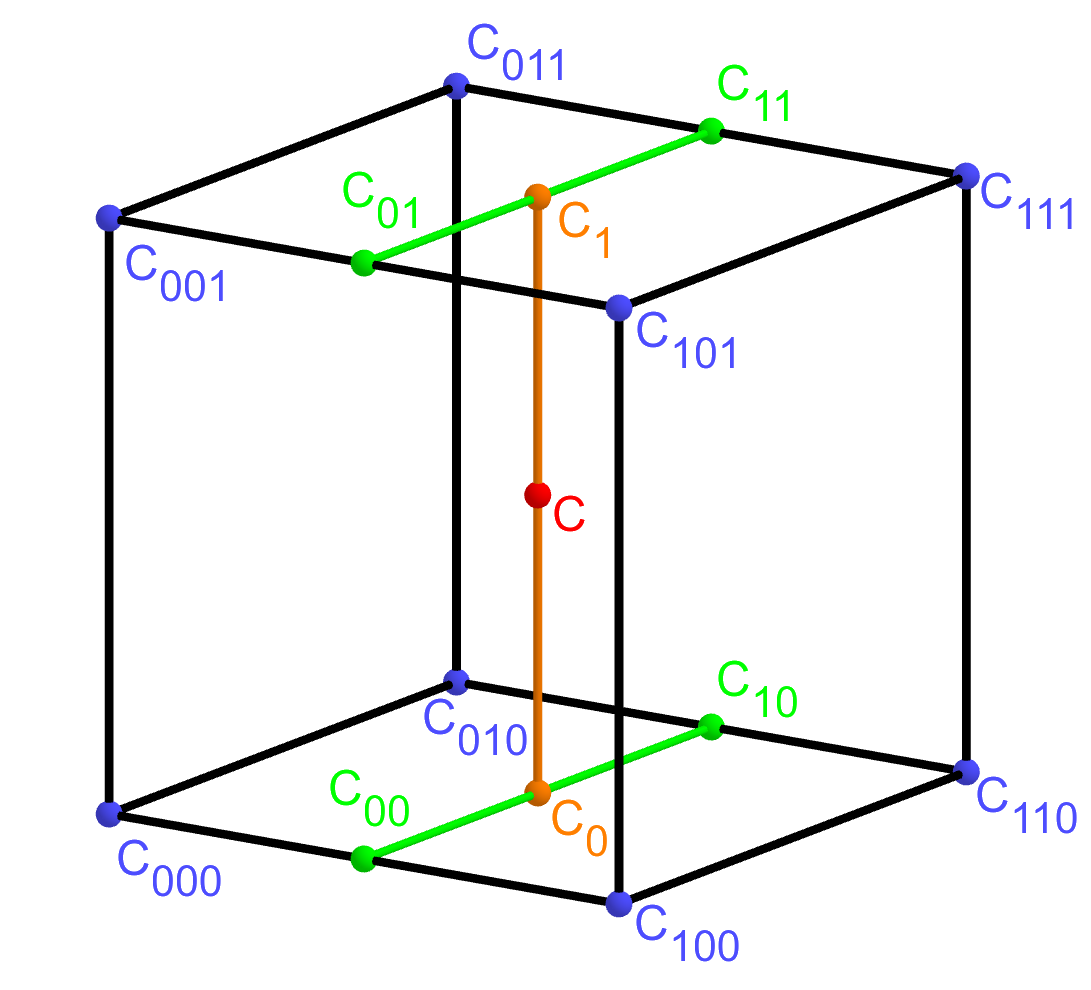
\includegraphics[width=0.5\textwidth]{trilinear.png}
					\caption{Visualization of trilinear interpolation as a~composition of linear interpolations (inspired by~\cite{trilinear1}). We want to interpolate the value in the red point~$\mathbf{C}$. First we interpolate between the four pairs of blue points sharing the last two indices along the $x$\protect\nobreakdash-axis (Eq.~\ref{eq:linterpol}), then between the two pairs of the resulting green points along the $y$\protect\nobreakdash-axis (Eq.~\ref{eq:linterpol2}) and finally between the two resulting orange points along the $z$\protect\nobreakdash-axis to get the final red value (Eq.~\ref{eq:linterpol3}).}
					\label{fig:trilin}
				\end{figure}
					
				\noindent We can also write
					\begin{eqnarray}
						\label{eq:trilingeo}
						\widehat{f}(\mathbf{C}) = \sum_{i,j,k \in \{0,1\}} t_x^i t_y^j t_z^k f(\mathbf{C}_{ijk}),\\
						t_\alpha \stackrel{\text{def}}{=} \begin{pmatrix}t_\alpha^0\\ t_\alpha^1\end{pmatrix} = \begin{pmatrix}1-\alpha_d\\ \alpha_d\end{pmatrix},
					\end{eqnarray}
				where $\alpha \in \{x,y,z\}$ is an index. This gives a~nice geometric interpretation to the trilinear interpolation as shown in \cref{fig:trilin2}. From this form and the figure, it is apparent that the final interpolated value does not depend on the order of axes along which we perform linear interpolations (see \cref{fig:trilin}). Furthermore, we can write $\widehat{f}(\mathbf{C})$ as a~polynomial:
					\begin{equation}
						\label{eq:trilinpoly}
						\widehat{f}(\mathbf{C}) = \sum_{\alpha,\beta,\gamma \in \{0,1\}}\sum^{\alpha}_{i=0}\sum^{\beta}_{j=0}\sum^{\gamma}_{k=0} 	(-1)^{(\alpha-i)+(\beta-j)+(\gamma-k)} f(\mathbf{C}_{ijk}) x_d^\alpha y_d^\beta z_d^\gamma.
					\end{equation}
				We take advantage of this form when generalizing trilinear interpolation to irregular grid in section~\ref{sec:interpol}.
					%\begin{equation}
					%	\widehat{f}(C) = (1-x_d) (1-y_d) (1-z_d) f(C_{000}) + (1-x_d) (1-y_d) z_d f(C_{001}) + (1-x_d) y_d (1-z_d) f(C_{010}) + (1-x_d) y_d z_d f(C_{011}) + x_d (1-y_d) (1-z_d) f(C_{100}) + x_d (1-y_d) z_d f(C_{101}) + x_d y_d (1-z_d) f(C_{110}) + x_d y_d z_d f(C_{111})
					%\end{equation}
					
				\begin{figure}
					\centering
					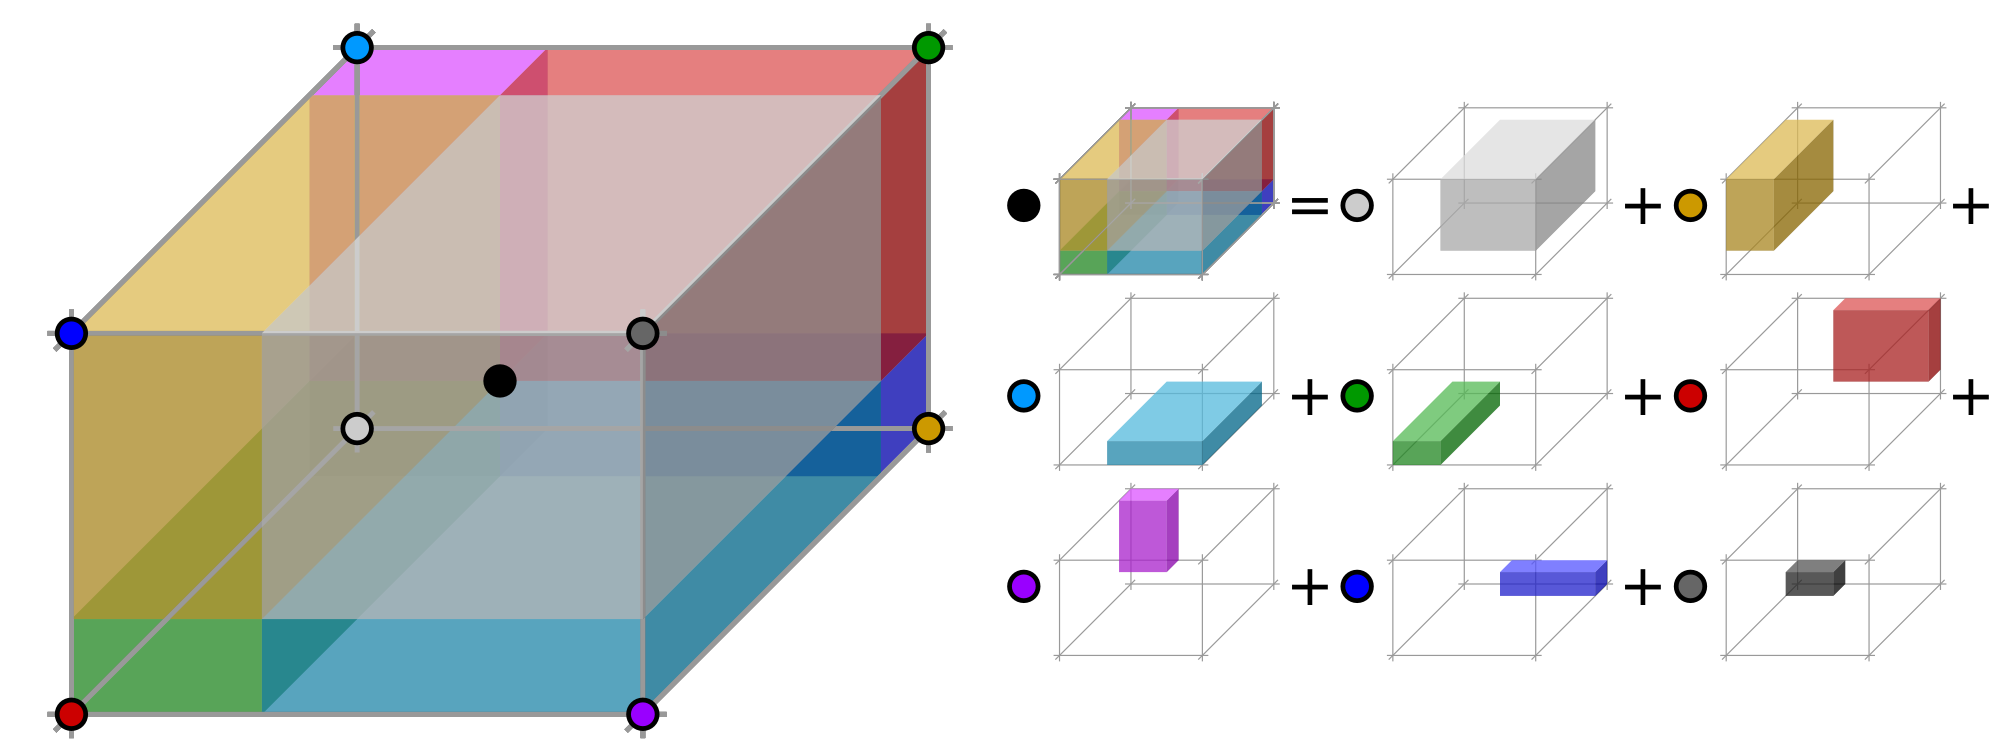
\includegraphics[width=\textwidth]{trilinear2.png}
					\caption{Geometric interpretation of trilinear interpolation as expressed in Equation~\ref{eq:trilingeo}. The colored dots represent the values in given points and the colored boxes represent the volume in the opposite corner by which the corresponding values are multiplied. The black dot represents the interpolated value which is multiplied by the entire volume~\cite{trilinear}.}
					\label{fig:trilin2}
				\end{figure}
				
				\red{Maybe a~citation here, although I am not sure it is necessary since it could be considered common knowledge. The last two equations are my own (but I'm not sure that's worth mentioning unless there's a citation).}